%% Document-wide settings.
\documentclass[letterpaper]{article}
\title{Poaky documentation}
\author{Thomas HOULLIER} 

\usepackage[colorlinks=true, allcolors=blue,
            hyperfootnotes=false,
            pdfauthor={Thomas HOULLIER},
            pdftitle={Poaky documentation},
	    pdfkeywords={Optical design, Raytracing, C++}]
            {hyperref} % Links for ref/cite.

%% Loading packages
\usepackage{amsmath} % For cases in equations.
\usepackage{amsfonts} % For maths sets.
\usepackage{amssymb} % Square symbol for QED
\usepackage{physics} % For \abs{} and \norm{}.
\usepackage[inkscapelatex=false]{svg} %svg graphics
\usepackage{siunitx} % units formatting

\usepackage[backend=biber,style=numeric,citestyle=numeric-comp,maxcitenames=99,dateabbrev=false]{biblatex}
\addbibresource{biblio.bib}
\usepackage{setspace} % Bibliography spacings
\DeclareSourcemap{
  \maps[datatype=bibtex]{
    \map[overwrite]{
      \step[fieldsource=doi, final]
      \step[fieldset=url, null]
      \step[fieldset=eprint, null] }}}
\setcounter{biburllcpenalty}{7000} % break long url in bibliography
\setcounter{biburlucpenalty}{8000}
\renewcommand*{\bibfont}{\footnotesize} % bibliography font size
% Format of biblatex urldate in the bibliography.
\DeclareFieldFormat{urldate}{%
  Visited on \thefield{urlday}\addspace%
  \mkbibmonth{\thefield{urlmonth}}\addspace%
  \thefield{urlyear}\isdot}
\usepackage[ruled,vlined]{algorithm2e} % Algorithms.
\DontPrintSemicolon
\SetKwInOut{Input}{Input}\SetKwInOut{Output}{Output}
\usepackage{mathtools} % Ceiling function.
\usepackage{outlines} % Nest lists.
\usepackage{interval} % Writing intervals.
\usepackage[font={footnotesize,sf}]{caption} %Caption for figures in minipages.
\usepackage{floatrow}
% Figure captions always below. Figures always centered.
\floatsetup[figure]{capposition=bottom,objectset=centering}
\usepackage{wrapfig} %Wrapping figure with text.
\usepackage{stmaryrd} % Double brackets for integers interval.
\usepackage{doi} % Hyperlink DOI
\usepackage{etoolbox} %Ragged right bibliography.
\usepackage{color, colortbl} % Coloring rows in tables.
\usepackage{subcaption} % Subfigures.
\usepackage{pdfpages} % Include PDF pages.
\usepackage{epigraph} % Quotations at beginning of chapters.
\setlength\epigraphwidth{.8\textwidth}
\usepackage[acronym,nonumberlist,nogroupskip,nopostdot]{glossaries} % Glossary for acronyms.
\renewcommand*{\glstextformat}[1]{\textcolor{black}{#1}} % No color on links for abbrev.

\DeclarePairedDelimiter{\ceil}{\lceil}{\rceil} % Ceiling function.
\DeclarePairedDelimiter{\floor}{\lfloor}{\rfloor} % Floor function.

\DeclareMathOperator*{\argmin}{argmin}

\setcounter{tocdepth}{3} % Table of content depth
\setcounter{secnumdepth}{3} % Section numbering depth

% Non-breaking around footnotes.
\makeatletter
\let\Footnote\footnote
\def\pst@@killglue{\unskip\ifdim\lastskip>\z@\expandafter\pst@@killglue\fi}
\def\footnote{\pst@@killglue\Footnote}
\makeatother

% More space below equations
\appto\normalsize{\belowdisplayshortskip=\belowdisplayskip}

% Rewrite month codes in bibliography
\DeclareSourcemap{
  \maps[datatype=bibtex]{
    \map[overwrite]{
      \step[fieldsource=month, match=\regexp{\A(j|J)an(uary)?\Z}, replace=1]
      \step[fieldsource=month, match=\regexp{\A(f|F)eb(ruary)?\Z}, replace=2]
      \step[fieldsource=month, match=\regexp{\A(m|M)ar(ch)?\Z}, replace=3]
      \step[fieldsource=month, match=\regexp{\A(a|A)pr(il)?\Z}, replace=4]
      \step[fieldsource=month, match=\regexp{\A(m|M)ay\Z}, replace=5]
      \step[fieldsource=month, match=\regexp{\A(j|J)un(e)?\Z}, replace=6]
      \step[fieldsource=month, match=\regexp{\A(j|J)ul(y)?\Z}, replace=7]
      \step[fieldsource=month, match=\regexp{\A(a|A)ug(ust)?\Z}, replace=8]
      \step[fieldsource=month, match=\regexp{\A(s|S)ep(tember)?\Z}, replace=9]
      \step[fieldsource=month, match=\regexp{\A(o|O)ct(ober)?\Z}, replace=10]
      \step[fieldsource=month, match=\regexp{\A(n|N)ov(ember)?\Z}, replace=11]
      \step[fieldsource=month, match=\regexp{\A(d|D)ec(ember)?\Z}, replace=12]}}}

% Footnotes marker color
\renewcommand\thefootnote{\textcolor{blue}{\arabic{footnote}}}

\pdfsuppresswarningpagegroup=1 % Silence warnings about pagegroups for figures.
\pdfminorversion=6 % PDF version 1.6 since we include articles in 1.6.

% Allow an extra pass to fix overfull hboxes by allowing more whitespace.
\emergencystretch=1em

% Page numbering and copyright notice.
\usepackage{fancyhdr}
\usepackage{lastpage}

\fancypagestyle{FirstPage}{
\fancyhf{} % Clear footer.
\rfoot{\thepage \hspace{1pt} of \pageref*{LastPage}}
\renewcommand{\headrulewidth}{0pt} % Remove rule at top of page
\lfoot{\href{https://creativecommons.org/licenses/by/4.0/}
       {\includesvg[inkscapelatex=false,height=14pt]{images/ccby.svg}}}
\lhead{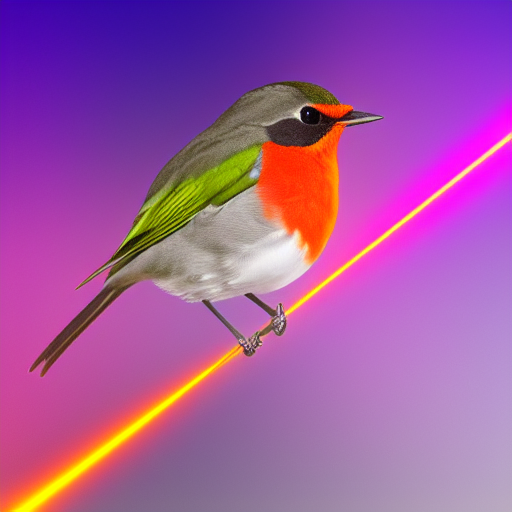
\includegraphics[height=64pt]{images/robintrace-logo.png}}
\chead{RobinTrace}
}

\fancypagestyle{plain}{
\fancyhf{} % Clear footer.
\rfoot{\thepage \hspace{1pt} of \pageref*{LastPage}}
\renewcommand{\headrulewidth}{0pt} % Remove rule at top of page
}

% Version history
\usepackage{vhistory}

% Keywords
\providecommand{\keywords}[1]{\textbf{Keywords --} #1}

% Glossary
\makeglossaries
\loadglsentries{glossary/glossary.tex}

\usepackage{fontawesome} %inline icons
\usepackage{xcolor}
\usepackage{listings} % Code listings
\definecolor{codeback}{rgb}{0.99,0.99,0.98}
\definecolor{codecomment}{HTML}{0588fc}
\definecolor{codekeyword}{HTML}{af5f00}
\definecolor{codestring}{HTML}{ffa07a}
\lstdefinestyle{mystyle}{
  backgroundcolor=\color{codeback},
  commentstyle=\color{codecomment},
  keywordstyle=\color{codekeyword},
  stringstyle=\color{codestring},
  basicstyle=\ttfamily\footnotesize,
  breakatwhitespace=false,         
  breaklines=true,                 
  captionpos=b,                    
  keepspaces=true,                 
  numbers=left,                    
  numbersep=5pt,                  
  showspaces=false,                
  showstringspaces=false,
  showtabs=false,                  
  tabsize=2}
\lstset{style=mystyle}

\usepackage[capitalise,nameinlink]{cleveref} % Include eg. "Fig." in front of figures.
\crefname{algorithm}{Alg.}{Algs.}
\crefname{table}{Tab.}{Tabs.}
\crefname{equation}{Eq}{Eqs.}
% Equation cross-references.
%\creflabelformat{equation}{#2#1#3}
\crefformat{equation}{(#2Eq.\thinspace#1#3)}

% No parentheses in equation labels.
%\newtagform{noparen}{}{}
%\usetagform{noparen}



% Document
\begin{document}
\frenchspacing
\date{v1.0 -- \today}
\maketitle
\thispagestyle{FirstPage}

\begin{abstract}
We document the development of Poaky, a piece of software for raytracing
through optical systems. Poaky is implemented in C++.
\end{abstract}

\keywords{Optical design, Raytracing, C++}

\begin{versionhistory}
\vhEntry{1.0}{\today}{TH}{creation}
\end{versionhistory}
\setcounter{table}{0} % Reset the table counter.

\tableofcontents
\printglossary[type=\acronymtype,style=index]
\pagestyle{plain}

\section{Introduction}

\section{Definitions and conventions}
We provide the conventions that were used. They are choices
on our part. Some details may differ from the choices made in
other tools.

\subsection{Raytracing sequence}
Poaky deals with optical systems represented as a sequence of optical
objects which operate on rays of light. The objects are of two main types,
optical surfaces and geometric propagators through some medium in between
surfaces (which we call \emph{transfer}). The sequence in which rays of light
interact with either surfaces or transfers is known a priori. The simulation of
the propagation of rays through such a sequence of objects is known as
\emph{sequential raytracing}. This discipline is linked with the more well
known raytracing for rendering, though they seem to have developed more
or less autonomously.

\subsection{Local coordinate system} \label{sec:LCS}
Each surface corresponds to an implicit \gls{LCS}.
This coordinate system may be described as containing (\cref{fig:LCS}):

\begin{itemize}
\item An apex $A$, which is the origin.
\item A local $z=0$ plane, which we often refer to as the \emph{local plane}.
\item A set of axes (implicit).
\end{itemize}

\begin{figure} \caption{\label{fig:LCS} LCS diagram.}
\includesvg[height=.2\textheight, width=.9\textwidth, keepaspectratio]
           {images/conventions/LCS.svg}
\end{figure}

We call the \gls{LCS} implicit because the actual meaning of the data
expressed in it depends on the interplay between surface defition, ray
transfer equations and ray operation conventions.

\subsection{Rays in local coordinate systems}

\begin{figure} \caption{\label{fig:ray-in-LCS} Ray definition
in \gls{LCS}.}
\includesvg[height=.2\textheight, width=.9\textwidth, keepaspectratio]
           {images/conventions/ray_in_LCS.svg}
\end{figure}

Given a \gls{LCS}, a ray may be defined by (\cref{fig:ray-in-LCS}):
\begin{itemize}
\item $P = \begin{bmatrix}x \\ y \\ z \end{bmatrix}$, a point.
\item $\overrightarrow{V} = \begin{bmatrix} l \\ m \\ n \end{bmatrix}$, a unit
vector oriented by the light propagation.
\end{itemize}

The components of $\overrightarrow{V}$ are often called in optics by the name
\emph{direction cosines} \cite{mathworld:direction-cosine}. Indeed, given the
basis vectors of our \gls{LCS}: $(\hat{x}, \hat{y}, \hat{z})$, the vector
$\overrightarrow{V}$ can be described by the angles $(\alpha, \beta, \gamma)$
between itself and each basis vector respectively. These angles may be defined
by \cref{eq:direction-cosines}.

\begin{equation} \label{eq:direction-cosines}
\begin{cases}
\cos(\alpha) &= \frac{\overrightarrow{V} \cdot \hat{x}}
                     {\abs{\overrightarrow{V}}} \\
\cos(\beta) &= \frac{\overrightarrow{V} \cdot \hat{y}}
                    {\abs{\overrightarrow{V}}} \\
\cos(\gamma) &= \frac{\overrightarrow{V} \cdot \hat{z}}
                     {\abs{\overrightarrow{V}}}
\end{cases}
\end{equation}

The points $(x_t, y_t, z_t)$ describing the ray trajectory through the use of a parameter $t$
are described by \cref{eq:ray-trajectory}.

\begin{equation} \label{eq:ray-trajectory}
\begin{bmatrix}
x_t \\ y_t \\ z_t
\end{bmatrix} =
\begin{bmatrix}
x + t \cdot l \\
y + t \cdot m \\
z + t \cdot n
\end{bmatrix}
\end{equation}

\subsection{Ray transfer conventions}
The \lstinline{transfer} objects take rays defined by a point located
anywhere and propagate them to rays resting on the local plane of the
next surface's \gls{LCS}. Surfaces operate under the assumption that
the input rays have a $z=0$ coordinate, and may leave the output rays
with any position. These assumptions are put in place for the management
of complex ray/surface intersections (which are not implemented in the
present version).

\section{Functional description}
This section defines the program's objects and their associated
operations. The style is minimal and close to the computations. For
the rationale sustaining the computation and complementary information,
see the justification section (\cref{sec:justification}).

\subsection{base}
Some base types are useful throughout the program. These are detailed in this
section.

\subsubsection{Point3}
\lstinline{Point3} are points in 3D space. They are described by $(x, y, z)$
coordinates.

\subsubsection{UVec3}
\lstinline{UVec3} are unit vectors in 3D space.

\subsection{ray}
\lstinline{ray} objects are the centerpiece of the simulation. They must be
lightweight objects.  \lstinline{ray} holds a position and a unit vector in the
direction and orientation of the propagation of light:

\begin{itemize}
\item \lstinline{Point3 p}: A point.
\item \lstinline{UVec3 v}: A vector, oriented by light propagation.
\end{itemize}

The interpretation of the data contained in a \lstinline{ray} is dependent
on context, as they are expressed in the current surface coordinate system.

In addition to their geometric definition, rays also hold a status code.
This code signals whether raytracing operations were successful, and if
not, which error case was encountered. There is no guarantee on the value
of the ray point and vector when the status code signals an error.

\begin{itemize}
\item \lstinline{int code}: Status code.
\end{itemize}

The status codes are defined in \cref{tab:ray-status-codes}.

\begin{table} \caption{\label{tab:ray-status-codes} Ray status codes.}
\begin{tabular}{| c | l |} \hline
\textbf{Code} & \textbf{Meaning} \\ \hline
0 & Success, the ray is valid.\\ \hline
1 & Sphere intersection: No intersection. \\ \hline
2 & Sphere intersection: Intersection beyond first hemisphere. \\ \hline
3 & refract: \gls{TIR} \\ \hline
4 & transfer: ray is parallel to the new local plane. \\
\hline \end{tabular}
\end{table}

\subsection{rop}
\lstinline{rop} are ray operations.

\subsubsection{reflect}
\lstinline{reflect} is a ray operation which applies the law of specular
reflection \cite{wiki:specular-reflection}. The ray direction is modified in
place. The normal vector $\overrightarrow{N}$ is already computed. There are
no error cases. The operation is illustrated on \cref{fig:reflect}.

\begin{equation}
\begin{bmatrix} l_r \\ m_r \\ n_r \end{bmatrix} =
\begin{bmatrix} l \\ m \\ n \end{bmatrix} - 2 \cdot
\overrightarrow{N} \cdot \left( \overrightarrow{N} \cdot
\begin{bmatrix} l \\ m \\ n \end{bmatrix} \right)
\end{equation}

\begin{figure} \caption{\label{fig:reflect} reflect operation quantities.}
\includesvg[height=.2\textheight, width=.9\textwidth, keepaspectratio]
           {images/shape/abstract-reflect.svg}
\end{figure}

\subsubsection{refract}
\lstinline{refract} is a ray operation applying the Snell law of refraction
\cite{wiki:snell-refraction}. The ray direction is modified in place.  We use
Xavier Bec's formula (\cite{Marrs:2021} p.105, \cite{Bec:1997}) for efficiency.
The operation is illustrated on \cref{fig:refract}.

\begin{figure} \caption{\label{fig:refract} refract operation quantities.}
\includesvg[height=.2\textheight, width=.9\textwidth, keepaspectratio]
           {images/shape/abstract-refract.svg}
\end{figure}

Let,

\begin{itemize}
\item $n_1$ the incident medium refraction index,
\item $n_2$ the output medium refraction index,
\item $n_r = \frac{n_1}{n_2}$,
\item $\overrightarrow{i}$ the unit incident ray direction,
\item $\overrightarrow{N}$ the unit surface normal vector,
\item $\overrightarrow{t}$ the unit refracted ray direction.
\end{itemize}

\begin{equation}
\begin{split}
&c_1 = - \overrightarrow{i} \cdot \overrightarrow{N} \\
&w = n_r \cdot c_1 \\
&c_{2m} = (w - n_r) \cdot (w + n_r)
\end{split} \end{equation}

At this stage, if $c_{2m} < -1$, then we set the \gls{TIR} ray
error code and the computation stops. Otherwise we proceed with
the computation of the refracted ray direction.
with:

\begin{equation} \label{eq:bec-formula}
\overrightarrow{t} = n_r \cdot \overrightarrow{i} +
(w - \sqrt{1 + c_{2m}}) \cdot \overrightarrow{N}
\end{equation}

\subsubsection{transfer} \label{sec:transfer}
A transfer defines a new \gls{LCS} to propagate the ray to.  The transfer
operation operates a change of basis and an intersection with the newly defined
local plane.

\paragraph{Definition}
Let,
\begin{itemize}
\item LCS1 the starting \gls{LCS} defined by its origin and basis vectors
$(A_1, \hat{x_1}, \hat{y_1}, \hat{z_1})$,
\item LCS2 the \gls{LCS} defined by the transfer operation, 
$(A_2, \hat{x_2}, \hat{y_2}, \hat{z_2})$.
\end{itemize}

The transfer operation is characterized by
\begin{itemize}
\item $B \in \mathbb{R}^{3 \times 3}$: A rotation matrix between the basis
vectors of LCS1 and LCS2. $B$ is orthogonal by definition,
hence $B^{-1} = B^\top$ \cite{wiki:rotation-matrix}.
\item $\overrightarrow{D} \in \mathbb{R}^3$: A translation vector between
LCS1 and LCS2.
\end{itemize}

The coordinates of the origin and basis vectors of LCS2 are expressed in
the original LCS1 coordinates by the following relations.

\begin{equation} \begin{cases}
A_2 = B \cdot \overrightarrow{D} \\
\hat{x_2} = B \cdot \hat{x_1} \\
\hat{y_2} = B \cdot \hat{y_1} \\
\hat{z_2} = B \cdot \hat{z_1}
\end{cases} \end{equation}

Which is to say, LCS2 is obtained from LCS1 by first applying the rotation $B$
and then translating the origin by $\overrightarrow{D}$, with
$\overrightarrow{D}$ expressed in the rotated coordinates. The change of basis
is illustrated on \cref{fig:transfer-definition}.

\begin{figure} \caption{\label{fig:transfer-definition}
Definition of the transfer between LCS1 and LCS2.}
\includesvg[height=.2\textheight, width=.9\textwidth, keepaspectratio]
           {images/shape/transfer-definition.svg}
\end{figure}

\paragraph{Operation}
The \lstinline{transfer} operation can be decomposed as two successive
operations on the ray:

\begin{itemize}
\item A change of basis from LCS1 to LCS2.
\item A ray intersection with the local plane of LCS2.
\end{itemize}

Let a ray expressed in LCS1 with starting point and direction
$(P_1, \overrightarrow{V_1})$. We first operate a change of basis from LCS1
to LCS2, which gives the coordinates $(P_2, \overrightarrow{V_2})$.

\begin{equation} \begin{cases}
P_2 = \begin{bmatrix} x_2 \\ y_2 \\ z_2 \end{bmatrix}
    = B^{-1} \cdot P_1 - \overrightarrow{D} \\
\overrightarrow{V_2} = \begin{bmatrix} l_2 \\ m_2 \\ n_2 \end{bmatrix}
  = B^{-1} \cdot \overrightarrow{V_1}
\end{cases} \end{equation}

We signal an error in the case $n_2 = 0$. This case corresponds to the
ray being parallel to the local plane of LCS2. We operate the intersection
of the ray with the LCS2 local plane next. The result ray is
$(P_3, \overrightarrow{V_3})$. The operation is illustrated by
\cref{fig:transfer-operation}.

\begin{equation} \begin{cases}
\overrightarrow{V_3} = \overrightarrow{V_2} \\
t = - \frac{z_2}{n_2} \\
P_3 = \begin{bmatrix} x_2 + t \cdot l_2 \\
                      y_2 + t \cdot m_2 \\
                      0 \end{bmatrix}
\end{cases} \end{equation}

\begin{figure} \caption{\label{fig:transfer-operation}
Illustration of the transfer operation on a ray.}
\includesvg[height=.2\textheight, width=.9\textwidth, keepaspectratio]
           {images/shape/transfer-operation.svg}
\end{figure}

\subsection{shape}
Shapes are an abstract concept specifying two operations:

\begin{itemize}
\item \lstinline{intersect}: Intersect a ray with the shape.
\item \lstinline{normal}: Provide a normal vector at the current ray
      position.
\end{itemize}

\paragraph{intersect}
The intersection operation takes a \lstinline{ray} expressed in the current
surface coordinate system with point on the local plane. It propagates
the ray until it hits the first encountered part of the shape. It modifies
the ray in-place. The modified ray is still expressed in the same current
coordinate system. This operation is illustrated on
\cref{fig:abstract-rayinter}.

\begin{figure} \caption{\label{fig:abstract-rayinter} Illustration of the
abtract intersect operation for a shape on a ray.}
\includesvg[height=.2\textheight, width=.9\textwidth, keepaspectratio]
           {images/shape/abstract-rayinter.svg}
\end{figure}

\paragraph{normal}
The normal operation provides a normal vector at the ray's current
position on the shape. The normal vector is expressed in the surface
LCS. The normal vector is a unit vector. The normal vector is oriented
with a $\hat{z}$ component of opposite sign to that of the ray's vector,
\textit{ie} the normal vector is in the opposite half-plane to the incident
ray. The normal operation is illustrated on \cref{fig:abstract-normal}. Error
cases can in theory happen due to numerical issues, they should be very rare.

\begin{figure} \caption{\label{fig:abstract-normal} Illustration of the
abstract normal operation for a shape and a ray.}
\includesvg[height=.2\textheight, width=.9\textwidth, keepaspectratio]
           {images/shape/abstract-normal.svg}
\end{figure}

\subsubsection{plane}
\paragraph{Definition}
A \lstinline{plane} is the local $z=0$ plane in the current \gls{LCS}.
It is specified implicitely.

\paragraph{intersect}
The input ray is already on the local plane. We do \emph{nothing} and cannot
fail.

\paragraph{normal}
The plane normal vector is trivial.
It is $\overrightarrow{N} = (0, 0, -\textrm{sign}(n))$.
There are no error cases.

\subsubsection{sphere}

\paragraph{Definition}
The \lstinline{sphere} is specified by:

\begin{itemize}
\item $R$: radius of curvature
\end{itemize}

The sphere is defined in the \gls{LCS} by \cref{eq:sphere-def}.

\begin{equation} \label{eq:sphere-def}
x^2 + y^2 + (z - R)^2 = R^2
\end{equation}

$R$ is the signed distance $\overline{AC}$, with $C$ the sphere center
(\cref{fig:sphere-def-lcs}). Only the hemisphere closest to the local plane
is considered as part of the \lstinline{sphere} shape.

\begin{figure} \caption{\label{fig:sphere-def-lcs} Sphere definition
in the LCS. Both signs of $R$ are represented.}
\includesvg[height=.2\textheight, width=.9\textwidth, keepaspectratio]
           {images/shape/sphere.svg}
\end{figure}

\textcolor{red}{TODO:
1. What happens if we define a sphere with R = 0? and for small R?
}

\paragraph{intersect}
The intersection between the input ray and the sphere is computed as
follows. The quantities involved are illustrated on \cref{fig:sphere-inter}.

\begin{figure} \caption{\label{fig:sphere-inter} Sphere intersection with
a ray diagram. The intersection point is $I$. The diagram is drawn arbitrarily
in the case $R<0$.}
\includesvg[height=.2\textheight, width=.9\textwidth, keepaspectratio]
           {images/shape/sphere-rayinter.svg}
\end{figure}

\begin{equation} \label{eq:ray-sphere-inter1}
\begin{cases}
b &= 2 (x \cdot l + y \cdot m - n \cdot R) \\
c &= x^2 + y^2 \\
\Delta &= b^2 - 4 c
\end{cases}
\end{equation}

If $\Delta \leq 0$, then no intersection exists. This is a ray error case.
Else, we continue with \cref{eq:ray-sphere-inter-tsol}.

\begin{equation} \label{eq:ray-sphere-inter-tsol}
t_\textrm{sol} = \frac{-b + \textrm{sign}(b) \cdot \sqrt{\Delta}}{2}
\end{equation}

Let $(x_I, y_I, z_I)$ the intersection point we wish to compute.

\begin{equation}
z_I = t_\textrm{sol} \cdot n
\end{equation}

If $\abs{z_I} \geq \abs{R}$, we have an intersection in the hemisphere furthest
from the local plane. This is another ray error case. Else, the remainder of
the solution can be computed.

\begin{equation} \begin{aligned}
x_I &= x + t_\textrm{sol} \cdot l \\
y_I &= y + t_\textrm{sol} \cdot m
\end{aligned} \end{equation}

\paragraph{normal}
The sphere normal vector is computed as follows. The ray rests on the previously
computed intersection point.

\begin{equation}
\overrightarrow{N} =
\frac{\textrm{sign}(n)}{R} \cdot
\begin{bmatrix} x \\ y \\ z - R \end{bmatrix}
\end{equation}

\subsection{lpart}

\subsubsection{tfr}

\subsubsection{surf}

\section{Proofs and justification}
\label{sec:justification}

Some implementation details require further justification and explanations.

\subsection{Ray intersection with a sphere}
Let us detail the computation of point $I$, the intersection between
a ray and a sphere. The ray has its point $P$ on the local plane
($z_P = 0$).
$I$ is both on the ray trajectory (parametrized by $t$) and on the sphere,
hence \cref{eq:sphere-intersect-just1}.

\begin{equation} \label{eq:sphere-intersect-just1}
\begin{cases}
x^2 + y^2 + (z - R)^2 = R^2 \\
x = x_P + t \cdot l \\
y = y_P + t \cdot m \\
z = t \cdot n
\end{cases}
\end{equation}

By substitution, we obtain \cref{eq:sphere-intersect-just2}.

\begin{equation} \label{eq:sphere-intersect-just2}
\begin{split}
&{x_P}^2 + 2 x_P \cdot t \cdot l + t^2
\cdot l^2 \\
+ &{y_P}^2 + 2 y_P \cdot t \cdot m + t^2
\cdot m^2 \\
+ &t^2 \cdot n^2 - 2 R \cdot t \cdot n + R^2
= R^2 \\
\iff &{x_P}^2 + {y_P}^2 \\
+ & 2 t (x_P \cdot l + y_P \cdot m - n \cdot R) \\
+ & t^2 (l^2 + m^2 + n^2) = 0
\end{split} \end{equation}

Since $\overrightarrow{V}$ is a unit vector, $(l^2 + m^2 + n^2) = 1$.
Hence we have a quadratic equation in $t$, \cref{eq:sphere-intersect-just3}.

\begin{equation} \label{eq:sphere-intersect-just3} \begin{cases}
t^2 + b \cdot t + c = 0 \\
b = 2 (x_P \cdot l + y_P \cdot m - n \cdot R) \\
c = {x_P}^2 + {y_P}^2
\end{cases} \end{equation}

The cases in \cref{eq:sphere-intersect-just4} are distinguished.

\begin{equation} \label{eq:sphere-intersect-just4} \begin{cases}
\Delta = b^2 - 4c & \\
\Delta < 0 & \text{no intersection} \\
\Delta = 0 & \text{one intersection (the ray is tangent to the sphere)} \\
\Delta > 0 & \text{two intersections can be found}
\end{cases} \end{equation}

We discard the case where no intersection is found. We also discard
the tangency case for two reasons. First, numerically, it cannot be checked
rigorously in our framework. Second, we see no application within our scope
that would exhibit this case nominally. These discarded cases are illustrated
in \cref{fig:sphere-inter-delta}.

\begin{figure} \caption{\label{fig:sphere-inter-delta} Sphere intersection
error cases on the sign of $\Delta$.}
\includesvg[height=.2\textheight, width=.9\textwidth, keepaspectratio]
           {images/shape/sphere-rayinter-errorcase-delta.svg}
\end{figure}

The two intersections are given by \cref{eq:sphere-intersect-just5}.

\begin{equation} \label{eq:sphere-intersect-just5} \begin{cases}
t_1 = \frac{-b + \sqrt{\Delta}}{2} \\
t_2 = \frac{-b - \sqrt{\Delta}}{2}
\end{cases} \end{equation}

We want the intersection to be the one closest to the local plane
(see the justification below), hence with minimal $\abs{z}$
(\cref{eq:sphere-intersect-just6}).

\begin{equation} \label{eq:sphere-intersect-just6} \begin{cases}
t_\textrm{sol} = \underset{t}{\mathrm{argmin}} \abs{t \cdot n} 
               = \underset{t}{\mathrm{argmin}} \abs{t} \\
t = \{ t_1, t_2 \}
\end{cases} \end{equation}

Hence, $t_\textrm{sol}$ is the solution with minimal absolute value.
$\abs{-b \pm \sqrt{\Delta}}$ is minimal iff
$-b$ and $\pm \sqrt{\Delta}$ are opposite in sign. Thus our
solution is \cref{eq:sphere-intersect-just7}.

\begin{equation} \label{eq:sphere-intersect-just7}
t_\textrm{sol} = \frac{-b + \textrm{sign}(b) \cdot \sqrt{\Delta}}{2}
\end{equation}

We can start applying $t_\textrm{sol}$ to the ray trajectory to find
the intersection point.

\begin{equation}
z_I = t_\textrm{sol} \cdot n
\end{equation}

The intersection could have happened in the hemisphere which we do
not want to consider. We consider \cref{eq:sphere-intersect-just8}.

\begin{equation} \label{eq:sphere-intersect-just8}
\begin{cases}
\abs{z_I} < \abs{R} & \text{Intersection in valid hemisphere} \\
\abs{z_I} \geq \abs{R} & \text{Intersection in wrong hemisphere}
\end{cases}
\end{equation}

We then assign an error case to $\abs{z_I} \geq \abs{R}$
(\cref{fig:sphere-inter-error-zi}).  If the intersection is in the right
hemisphere however, we can continue by computing the remaining point
coordinates \cref{eq:sphere-intersect-just9}.

\begin{equation} \label{eq:sphere-intersect-just9}
\begin{cases}
x_I &= x + t_\textrm{sol} \cdot l \\
y_I &= y + t_\textrm{sol} \cdot m
\end{cases} \end{equation}

\begin{figure} \caption{\label{fig:sphere-inter-error-zi} Sphere intersection
error case on the hemisphere being intersected.}
\includesvg[height=.2\textheight, width=.9\textwidth, keepaspectratio]
           {images/shape/sphere-rayinter-errorcase-zi.svg}
\end{figure}

$\square$

\paragraph{Intersection selection rationale}
\label{sec:sphere-intersection-selection}

We explain why we select the intersection solution that is closest to
the local plane. Notably, we do not want necessarily the \emph{first}
intersection with the hemisphere encountered by the ray in its propagation.

The hemisphere is defined as either \emph{concave} or \emph{convex} by its
radius and by the orientation of incoming rays. This determines
the intended optical interaction of the ray with the surface.  For instance, a
\emph{concave} mirror applies a converging optical power to incoming rays. All
the cases are listed in \cref{tab:sphere-definition-cases}.

\begin{table} \caption{\label{tab:sphere-definition-cases} Intended sphere
shape as seen by incoming rays.}
\begin{tabular}{| c | c | c |} \hline
-       & $n < 0$ & $n > 0$ \\ \hline
$R < 0$ & convex  & concave \\ \hline
$R > 0$ & concave & convex  \\
\hline \end{tabular} \end{table}

A ray at one of its two eventual points of intersection with a sphere can be
said to either \emph{exit} or \emph{enter} the sphere, along its own
propagation direction. The shape of the sphere as seen by the oriented incoming
ray is determined by the alternative between \emph{exitting} and
\emph{entering}.  The rays incoming onto a \emph{concave} sphere must intersect
the sphere at the point they are \emph{exitting} the sphere.  Conversely, the
rays incoming onto a \emph{convex} sphere must intersect the sphere at the
point they are \emph{entering} the sphere. \cref{tab:sphere-exit-entrance}
summarizes the intersection point we need.

\begin{table} \caption{\label{tab:sphere-exit-entrance} Intersection point
to compute for each case.}
\begin{tabular}{| c | c | c |} \hline
-       & $n < 0$   & $n > 0$  \\ \hline
$R < 0$ & entrance  & exit     \\ \hline
$R > 0$ & exit      & entrance \\
\hline \end{tabular} \end{table}

Consider that: \begin{itemize}
\item Out of the two eventual intersection points, one is \emph{exitting},
the other is \emph{entering}.
\item The ray, along its propagation (increasing $t$), must first \emph{enter}
the sphere and then \emph{exit}.
\end{itemize}

We note $t_\textrm{en}$ the parameter along the ray trajectory at the sphere
entrance, and $t_\textrm{ex}$ the parameter at the sphere exit. Necessarily,
we have $t_\textrm{ex} > t_\textrm{en}$. Incidentally, this allows assigning
either the entrance or exit to the $t_\textrm{sol}$ parameter
\cref{eq:sphere-intersect-just5}. This is another way of disambiguating the
solution $t_\textrm{sol}$, but we want to prove the solution is closest to the
local plane.

\begin{equation}
\begin{cases}
t_\textrm{ex} &= \frac{-b + \sqrt{\Delta}}{2} \\
t_\textrm{en} &= \frac{-b - \sqrt{\Delta}}{2}
\end{cases}
\end{equation}

The intersection point happens at $z = t \cdot n$, in each case we can
determine the order between $z_\textrm{ex} = t_\textrm{ex} \cdot n$ and
$z_\textrm{en} = t_\textrm{en} \cdot n$.

\begin{itemize}
\item $n>0$: $z_\textrm{ex} > z_\textrm{en}$
\item $n<0$: $z_\textrm{ex} < z_\textrm{en}$
\end{itemize}

By our definition of the sphere, any intersection point $z$ coordinate
has a sign given by the sign of $R$.

\begin{itemize}
\item $R>0$: $z>0$
\item $R<0$: $z<0$
\end{itemize}

Hence we can deduce an order between $\abs{z_\textrm{ex}}$ and
$\abs{z_\textrm{en}}$ depending on the case
(\cref{tab:sphere-intersection-zorder}).

\begin{table} \caption{\label{tab:sphere-intersection-zorder} 
Order in $\abs{z}$ of intersection points.}
\begin{tabular}{| c | c | c |} \hline
-       & $n < 0$   & $n > 0$  \\ \hline
$R < 0$ & $\abs{z_\textrm{en}} < \abs{z_\textrm{ex}}$ &
          $\abs{z_\textrm{en}} > \abs{z_\textrm{ex}}$     \\ \hline
$R > 0$ & $\abs{z_\textrm{en}} > \abs{z_\textrm{ex}}$ &
          $\abs{z_\textrm{en}} < \abs{z_\textrm{ex}}$ \\
\hline \end{tabular} \end{table}

Finally, we can conclude by crossing \cref{tab:sphere-exit-entrance}
and \cref{tab:sphere-intersection-zorder}, that the intersection point
we need to pick is always the one with minimal $\abs{z}$. Hence the
solution we need is always closest to the local plane.\footnote{Admittedly,
this justification is laborious. The reader can convince themselves
that the solution intersection is the one closest to the local plane just
by looking at the diagrams.}

\paragraph{b = 0 case}
Looking at \cref{eq:ray-sphere-inter-tsol}, it may seem numerically
unstable around $b = 0$ due to the term $\textrm{sign}(b) \cdot \sqrt{\Delta}$.

However, at this stage of the computation, we have
\cref{eq:sphere-inter-just10}.

\begin{equation} \label{eq:sphere-inter-just10} \begin{cases}
b^2 &= \Delta + 4 c \\
\Delta &> 0 \\
c &\geq 0
\end{cases} \end{equation}

Hence, $\abs{b}$ can only near zero when both $\Delta$ and $c$ are near zero.
Thus the term $\textrm{sign}(b) \cdot \sqrt{\Delta}$ may be numerically
unstable in sign, but is near zero in this region.

\subsection{General expression for a shape normal vector}
Given a shape in its \gls{LCS} defined by an equation $z = f(x, y)$,
we can compute the unit normal vector at point $(x, y)$ using
\cref{eq:gen-normal} \cite{mathworld:normal-vector}. Additionally
we orient the normal vector in the opposite half-plane to an incident
ray with a vector component $n$.

\begin{equation} \label{eq:gen-normal}
\overrightarrow{N} =
\frac{\textrm{sign}(n)}
     {\sqrt{1 + \left(\frac{\partial f}{\partial x}(x, y)\right)^2 +
                \left(\frac{\partial f}{\partial y}(x, y)\right)^2}}
\cdot
\begin{bmatrix}
\frac{\partial f}{\partial x}(x, y) \\
\frac{\partial f}{\partial y}(x, y) \\
-1
\end{bmatrix}
\end{equation}

\subsection{Sphere altitude formulation and first derivatives}
We formulate the sphere altitude in the $z = f(x, y)$ form. This form
is useful for hand calculations, plots, etc. We follow by deriving the
first derivatives in $x$ and $y$.

\paragraph{altitude}
The complete sphere is described by

\begin{equation}
\begin{split}
& x^2 + y^2 + (z - R)^2 = R^2 \\
\iff & (z - R)^2 = R^2 - x^2 - y^2 \\
\iff & \abs{z-R} = \sqrt{R^2 - x^2 - y^2}
\end{split} \end{equation}

Now, we consider only the first hemisphere $(\abs{z} < \abs{R})$, so
there are two cases depending on the sign of $R$. Moreover, by definition,
the sign of $z$ is the same as that of $R$.

\begin{equation} \begin{cases}
\abs{z - R} = -z + R & R \geq 0 \\
\abs{z - R} = z - R & R < 0
\end{cases} \end{equation}

For the $R \geq 0$ case, we have:

\begin{equation} \begin{split}
& R - z = \sqrt{R^2 -x^2 -y^2} \\
\iff & z = R \left( 1 - \sqrt{1 - \frac{x^2 + y^2}{R^2}} \right)
\end{split} \end{equation}

For the $R < 0$ case, we have:

\begin{equation} \begin{split}
& z - R = \sqrt{R^2 -x^2 -y^2} \\
\iff & z = R \left( 1 + \sqrt{1 - \frac{x^2 + y^2}{R^2}} \right)
\end{split} \end{equation}

The two cases can be reunited in the following formula, which is the
analytic expression of the sphere shape in our program \cref{eq:sphere-alt}.

\begin{equation} \label{eq:sphere-alt}
z = R \left( 1 - \textrm{sign}(R) \sqrt{1 - \frac{x^2 + y^2}{R^2}} \right)
\end{equation}

\paragraph{derivatives}
We compute the partial derivative with respect to $x$ of \cref{eq:sphere-alt}.

\begin{equation} \begin{split}
\frac{\partial z}{\partial x} & = 
\frac{\partial}{\partial x}
\left( -R \cdot \textrm{sign}(R) \sqrt{1 - \frac{x^2 + y^2}{R^2}} \right) \\
& = - \abs{R} \frac{\partial}{\partial x}
\left( \sqrt{1 - \frac{x^2 + y^2}{R^2}} \right) \\
& = \abs{R} \cdot \frac{1}{\sqrt{1 - \frac{x^2 + y^2}{R^2}}} \cdot
\frac{x}{R^2} \\
& = \frac{R \cdot \textrm{sign}(R) \cdot x}{R \sqrt{R^2 - x^2 -y^2}} \\
& = \frac{\textrm{sign}(R) \cdot x}{\sqrt{R^2 - x^2 -y^2}}
\end{split} \end{equation}

By symmetry, we find the partial derivative with respect to $y$, both
formulae are in \cref{eq:sphere-derivatives}.

\begin{equation} \label{eq:sphere-derivatives} \begin{cases}
\frac{\partial z}{\partial x} (x, y) =
\frac{\textrm{sign}(R) \cdot x}{\sqrt{R^2 - x^2 -y^2}} \\
\frac{\partial z}{\partial y} (x, y) =
\frac{\textrm{sign}(R) \cdot y}{\sqrt{R^2 - x^2 -y^2}} \\
\end{cases} \end{equation}

\subsection{Sphere normal vector}
We derive an efficient expression for the normal vector of a sphere at
an intersection point. Keep in mind that we already know the intersection
point on the shape. We arrive at the result from two (slightly) different
starting points.

\subsubsection{Analytic formulation}
We plug the partial derivatives \cref{eq:sphere-derivatives} into the general
normal vector formula \cref{eq:gen-normal}.

\begin{equation} \begin{split}
\overrightarrow{N} & = \frac{\textrm{sign}(n)}
{\sqrt{1 + \frac{x^2}{R^2 - x^2 - y^2} + \frac{y^2}{R^2 - x^2 - y^2}}} \cdot
\begin{bmatrix}
\textrm{sign}(R) \cdot x \mathbin{/} \sqrt{R^2 - x^2 - y^2} \\
\textrm{sign}(R) \cdot y \mathbin{/} \sqrt{R^2 - x^2 - y^2} \\
-1
\end{bmatrix} \\
& = \frac{\textrm{sign}(n) \cdot \textrm{sign}(R) \cdot
          \sqrt{R^2 - x^2 - y^2}}
         {\sqrt{R^2 - x^2 - y^2 + x^2 + y^2}} \cdot
\begin{bmatrix}
x \mathbin{/} \sqrt{R^2 - x^2 - y^2} \\
y \mathbin{/} \sqrt{R^2 - x^2 - y^2} \\
-\textrm{sign}(R)
\end{bmatrix} \\
& = \frac{\textrm{sign}(R)}{\abs{R}} \cdot \textrm{sign}(n) \cdot
\begin{bmatrix}
x \\ y \\
- \textrm{sign}(R) \sqrt{R^2 - x^2 - y^2}
\end{bmatrix} \\
& = \frac{\textrm{sign}(n)}{R} \cdot
\begin{bmatrix}
x \\ y \\
- \textrm{sign}(R) \sqrt{R^2 - x^2 - y^2}
\end{bmatrix}
\end{split} \end{equation}

With,

\begin{equation} \begin{cases}
\abs{z-R} = R - z & R \geq 0 \\
\abs{z-R} = z - R & R < 0
\end{cases} \end{equation}

Hence,

\begin{equation}
\abs{z-R} \cdot \textrm{sign}(R) = R - z
\end{equation}

Which leads us to the efficient expression for the sphere normal vector
\cref{eq:sphere-normal-anaformula}.

\begin{equation} \label{eq:sphere-normal-anaformula}
\overrightarrow{N} = \frac{\textrm{sign}(n)}{R} \cdot
\begin{bmatrix}
x \\ y \\ z - R
\end{bmatrix}
\end{equation}

\subsubsection{Geometric formulation}
The center of the sphere is $C = (0, 0, R)$. We know the intersection point
$I = (x, y, z)$.

The normal vector to the sphere is colinear to $\overrightarrow{CI}$.

\begin{equation}
\overrightarrow{CI} = \begin{bmatrix} x \\ y \\ z - R \end{bmatrix}
\end{equation}

Now we obtain a vector $\overrightarrow{N_i}$ by flipping $\overrightarrow{CI}$
opposite to the incident ray in the $\hat{z}$ direction.

Remember that,

\begin{equation} \begin{cases}
z - R \leq 0 & R \geq 0 \\
z - R > 0 & R < 0
\end{cases} \end{equation}

so we have,

\begin{equation} \begin{cases}
\overrightarrow{N_i} = \textrm{sign}(n) \cdot
\begin{bmatrix} x \\ y \\ z - R \end{bmatrix} & R \geq 0 \\
\overrightarrow{N_i} = - \textrm{sign}(n) \cdot
\begin{bmatrix} x \\ y \\ z - R \end{bmatrix} & R < 0 \\
\end{cases} \end{equation}

Which can be summarized as,

\begin{equation}
\overrightarrow{N_i} = \textrm{sign}(n) \cdot \textrm{sign}(R) \cdot
\begin{bmatrix} x \\ y \\ z - R \end{bmatrix}
\end{equation}

Now, we simply normalize the vector in order to obtain $\overrightarrow{N}$.

\begin{equation} \begin{split}
\overrightarrow{N} &= \frac{\textrm{sign}(n) \cdot \textrm{sign}(R)}
{\sqrt{x^2 + y^2 + (z-R)^2}} \cdot
\begin{bmatrix} x \\ y \\ z - R\end{bmatrix} \\
&= \frac{\textrm{sign}(n) \cdot \textrm{sign}(R)}{\abs{R}} \cdot
\begin{bmatrix} x \\ y \\ z - R\end{bmatrix}
\end{split} \end{equation}

The efficient expression for $\overrightarrow{N}$ is given by
\cref{eq:sphere-normal-geoformula}.

\begin{equation} \label{eq:sphere-normal-geoformula}
\overrightarrow{N} = \frac{\textrm{sign}(n)}{R} \cdot
\begin{bmatrix} x \\ y \\ z - R\end{bmatrix}
\end{equation}

\subsection{Reflection formula derivation}
We derive the reflection formula. See the illustration \cref{fig:reflect}.
Let: \begin{itemize}
\item The surface normal $\overrightarrow{N}$ at the ray intersection.
\item The incident ray unit vector $\overrightarrow{i}$.
\item The reflected ray unit vector $\overrightarrow{r}$.
\item $\theta_i$ the (unsigned) angle between $\overrightarrow{N}$ and
      $\overrightarrow{i}$.
\item $\theta_r$ the (unsigned) angle between $\overrightarrow{N}$ and
      $\overrightarrow{r}$.
\end{itemize}

We want to compute $\overrightarrow{r}$ as a function of $\overrightarrow{i}$
and $\overrightarrow{N}$.
We assume the laws of reflection, which essentially state that light
behaves as a billiard ball in its geometrical interaction with the surface:
\begin{itemize}
\item The reflected ray is in the plane spanned by $\overrightarrow{i}$ and
      $\overrightarrow{N}$ (\emph{plane of incidence}), and opposite to
      $\overrightarrow{i}$ with respect to $\overrightarrow{N}$.
\item $\theta_i = \theta_r$
\end{itemize}

\subsubsection{Algebraic derivation}
We produce a derivation similar to that of \cite{Glassner:1989} (p.131).

\textcolor{red}{TODO: derivation. Pay attention to the "opposite" condition
on angles.}

\section{Tests and benchmarks}
We document the rationale for tests performed on the components of the
software. We also detail a representative performance report.

\subsection{Tests}
Our rationale for testing is the following.

\begin{itemize}
\item Every function must be called at least once.
\item Every eventual error case and condition must be reached at least once.
\item The correctness is assessed on a few samples, through the means of
      either:
  \begin{itemize}
  \item Pinning the function under test to a reference function which
        is very clearly expressed with respect to the documentation.
  \item Pinning the function result to an externally computed result.
  \end{itemize}
\end{itemize}

As the development proceeds, we add cases arising from fixed bugs in order to
prevent regression.

\subsection{Performance report}
We provide benchmark results for the operations we wrote. The goal is
to indicate what order of magnitude of performance can be expected.

\subsubsection{Hypotheses and limitations}
We run each function on sizeable arrays of rays, one ray at a time.
The functions are evaluated independently. This may be unrepresentative of
a real raytracing computation flow where complex operations may be chained
on only a few rays. The operations are run on CPU on a single thread.

\subsubsection{Hardware}
We ran the benchmark on a Void Linux desktop computer, with kernel version
6.0.11\_1. We took no particular steps to configure the OS. The computer
has a AMD Athlon 3000G CPU and DDR4 RAM clocked at 2667 MT/s. We compiled
the benchmark with gcc 10.2.1 with the flags \lstinline{-march=native -O2}.

\subsubsection{Results}
The benchmark results are listed in \cref{tab:benchmark}.

\begin{table} \caption{\label{tab:benchmark} Benchmark results}
\begin{tabular} {| c | c | c |} \hline
\textbf{Operation} & \textbf{Mean timing per op (ns)} &
  \textbf{Standard deviation (ns)} \\ \hline
reflect & 2.2 & 0.3 \\ \hline
refract & 5.6 & 0.6 \\ \hline
transfer & 5.6 & 0.9 \\ \hline
standard.intersect & 5.6 & 0.6 \\ \hline
standard.normal & 5.9 & 0.9 \\ \hline
\end{tabular}\end{table}


\section{Notations}
\subsection{Multiplication and dot product}
The symbol $\cdot$ may refer to:
\begin{itemize}
\item Scalar multiplication
\item Scalar/Vector or Scalar/Matrix multiplication
\item Vector dot product
\end{itemize}

\subsection{Absolute value and 2-norm}
The unary operator notation $\abs{\cdot}$ may refer to:
\begin{itemize}
\item Absolute value of a scalar
\item 2-norm (or \emph{Euclidian} norm) of a vector
\end{itemize}

\subsection{Sign function}
We use a sign function, defined as in \cref{eq:sign-fun}.

\begin{equation} \label{eq:sign-fun}
\textrm{sign}(x) = \begin{cases}
1 & \text{if } x \geq 0 \\
-1 & \text{otherwise}
\end{cases} \end{equation}

\section{Glossary}
Some technical terms are recurring. They are specific either to this document
or to optical design and thus must be defined.

\subsection{Local plane}
The \emph{local plane} is the $z=0$ plane in a \gls{LCS} (\cref{sec:LCS}).

\subsection{Concave or Convex}
We must disambiguate what we mean by \emph{convex} and \emph{concave}, as other
conventions are used in other fields. These adjectives apply to surface
shapes, often in the context of raytracing as seen by incoming rays.
It refers to the sign of the curvature of the shape.  The two terms are
illustrated on \cref{fig:concave-convex}. A surface shape may be described as
convex/concave either globally or locally at the ray intersection point.

\begin{figure} \caption{\label{fig:concave-convex} Illustration of a
ray incoming onto a concave surface (left), and on a convex surface (right).}
\includesvg[height=.2\textheight, width=.9\textwidth, keepaspectratio]
           {images/glossary/concave-convex.svg}
\end{figure}


\appendix
\cleardoublepage

%% \include{appendices}

\apptocmd{\thebibliography}{\raggedright}{}{}
\begingroup
\setstretch{0.6}
\setlength\bibitemsep{0pt}
\printbibliography
\endgroup
\end{document}
